\begin{frame}{Tipos de metodologías de investigación en Cs}
 \begin{figure}[H]
    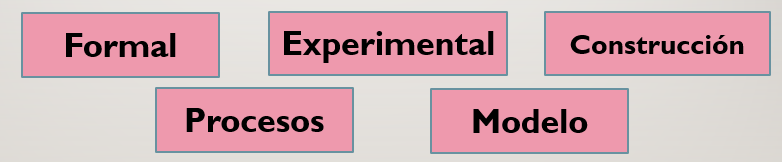
\includegraphics[scale=0.58]{images/figura2.PNG}
    \label{fig:boat1}
\end{figure}     
\end{frame}

\begin{frame}{Metodologías formales}
\begin{block}{}
\begin{itemize}
    \item Prueba hechos sobre algoritmos y sistemas. 
    \item Estas metodologías están más orientadas hacia la ciencia de la computación teórica. [1]
    \item Generalmente se ocupa del modelado y la abstracción. 

    \item Preguntas en  ciencias de la computación:
    \begin{itemize}
        \item Dado un problema X.
            \begin{itemize}
        \item ¿Qué tan difícil es resolverlo? (computabilidad)
        \item ¿Cuánto tiempo/espacio tarda? (complejidad)
        \item¿Cuáles son sus limitaciones? 
        \item Dado un formalismo, ¿qué puede expresar?
    \end{itemize}
    \end{itemize}
\end{itemize}
 \end{block} 
\end{frame}


\begin{frame}{Metodologías experimentales}
\begin{block}{}
\begin{itemize}
    \item Evaluar nuevas soluciones para problemas.[1]
    \item División:
    \begin{itemize}
        \item Fase exploratoria: Son las preguntas que se deben hacer sobre el sistema que se está evaluando. 
        \item Fase de evaluación: intentará responder estas preguntas. Un experimento bien diseñado comenzará con una lista de las preguntas que se espera que el experimento responda.
    \end{itemize}
\end{itemize}
 \end{block} 
\end{frame}

\begin{frame}{Metodologías de construcción}
\begin{block}{}
\begin{itemize}
    \item Consiste en construir un artefacto [1].
    \begin{itemize}
        \item Ya sea un artefacto físico o un sistema de software, para demostrar que es posible. 
    \end{itemize}
    \item Para ser considerada investigación, la construcción del artefacto debe ser nueva o debe incluir nuevas características que no se hayan demostrado anteriormente en otros artefactos.
\end{itemize}
 \end{block} 
\end{frame}

\begin{frame}{Metodologías de procesos}
\begin{block}{}
  \begin{itemize}
    \item Comprender los procesos utilizados para realizar tareas en  Ciencias de la computación. [1]
    \item Esta metodología se utiliza principalmente en las áreas de Ingeniería de software y Interfaz hombre-máquina, que se ocupan de la forma en que los humanos construyen y utilizan los sistemas informáticos. 
\end{itemize}  
 \end{block} 
\end{frame}

\begin{frame}{Metodologías de modelo}
\begin{block}{}
Los experimentos basados en un modelo se llaman simulaciones. Cuando se crea una descripción formal del modelo para verificar la funcionalidad o la corrección de un sistema, la tarea se denomina verificación de modelo.[1]
\begin{itemize}
    \item Centra en definir un modelo abstracto para un sistema real. Este modelo será mucho menos complejo que el sistema que modela y, por lo tanto.
    \item Permitirá al investigador comprender mejor el sistema y utilizar el modelo para realizar experimentos que no podrían realizarse en el propio sistema debido al costo o la accesibilidad. 
    \item Se utiliza a menudo en combinación con las otras cuatro metodologías.
\end{itemize} 
 \end{block} 
\end{frame}
